\begin{figure}[ht!]
    \begin{subfigure}{.5\textwidth}
    \centering
    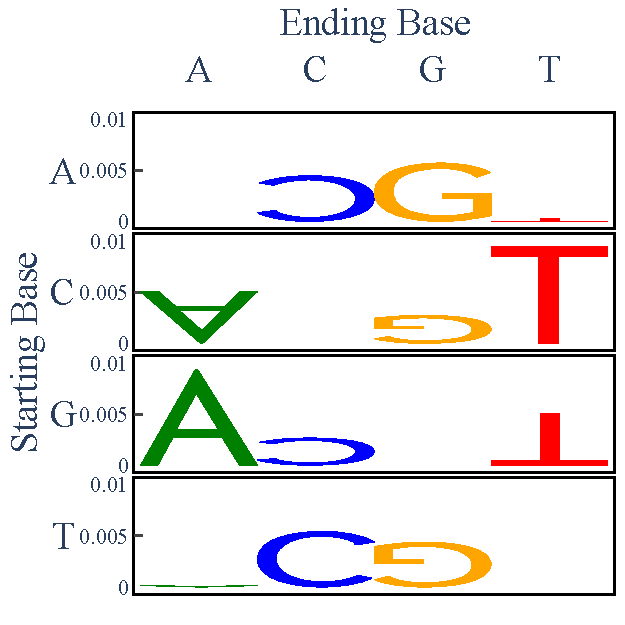
\includegraphics[scale=0.45]{graphics/spectra_Breast-AdenoCa.pdf}
    \caption{Breast-AdenoCa}
    \end{subfigure}
    ~
    \begin{subfigure}{.5\textwidth}
    \centering
    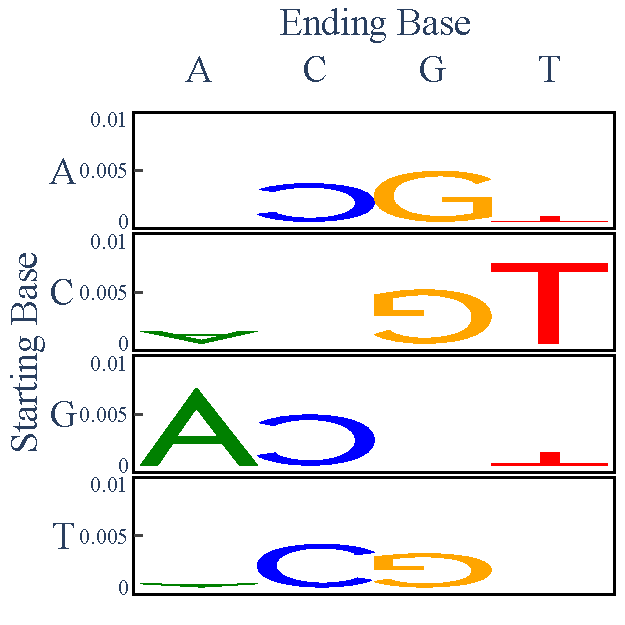
\includegraphics[scale=0.45]{graphics/spectra_Bone-Osteosarc.pdf}
    \caption{Bone-Osteosarc}
    \end{subfigure} \\
    % \vspace{0.1cm}
    
    \begin{subfigure}{.5\textwidth}
    \centering
    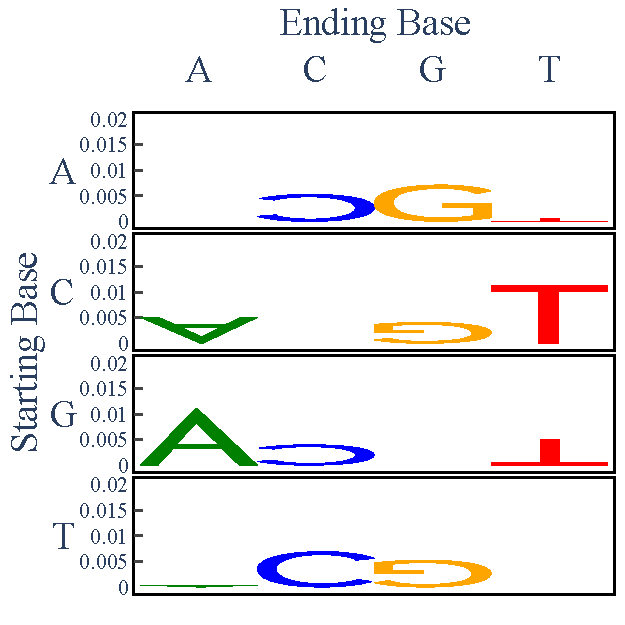
\includegraphics[scale=0.45]{graphics/spectra_CNS-Medullo.pdf}
    \caption{CNS-Medullo}
    \end{subfigure}
    ~
    \begin{subfigure}{.5\textwidth}
    \centering
    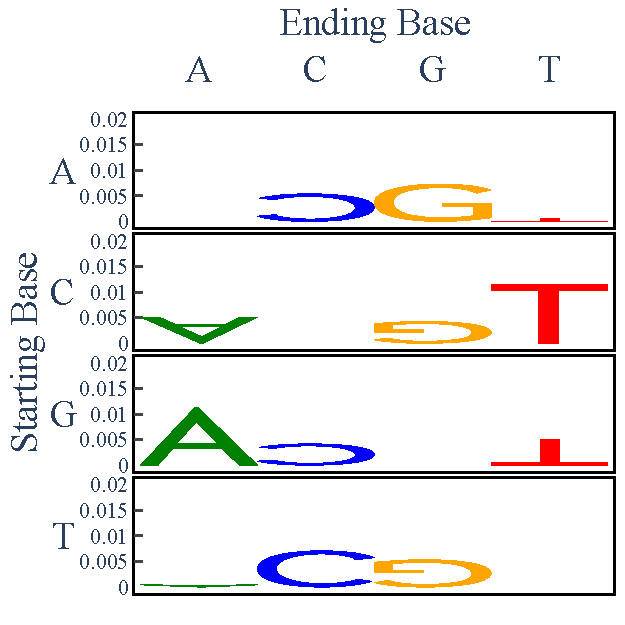
\includegraphics[scale=0.45]{graphics/spectra_CNS-PiloAstro.pdf}
    \caption{CNS-PiloAstro}
    \end{subfigure} \\
    % \vspace{0.1cm}
    
    \begin{subfigure}{.5\textwidth}
    \centering
    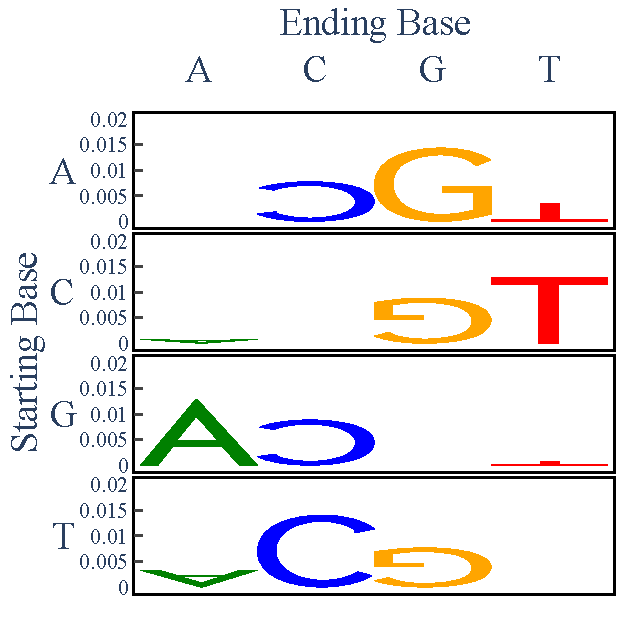
\includegraphics[scale=0.45]{graphics/spectra_Lymph-BNHL.pdf}
    \caption{Lymph-BNHL}
    \end{subfigure}
    ~
    \begin{subfigure}{.5\textwidth}
    \centering
    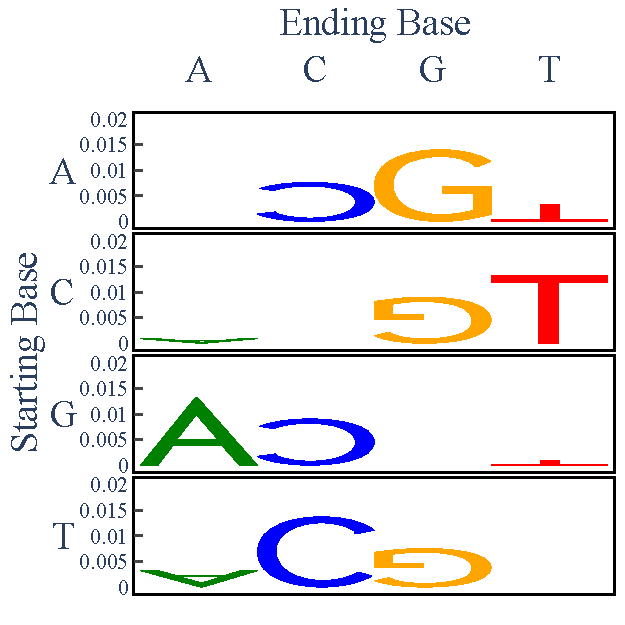
\includegraphics[scale=0.5]{graphics/spectra_Lymph-CLL.pdf}
    \caption{Lymph-CLL}
    \end{subfigure} \\
    % \vspace{0.1cm}
    
    \begin{subfigure}{.5\textwidth}
    \centering
    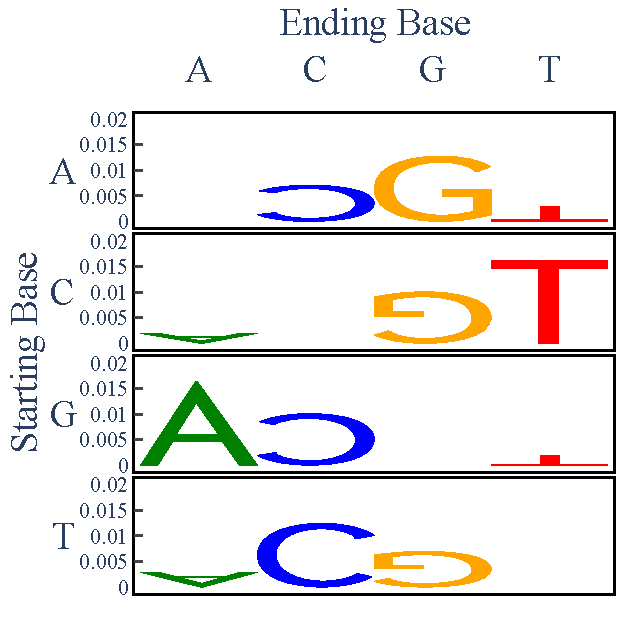
\includegraphics[scale=0.5]{graphics/spectra_Panc-Endocrine.pdf}
    \caption{Panc-Endocrine}
    \end{subfigure} 
    ~
    \begin{subfigure}{.5\textwidth}
    \centering
    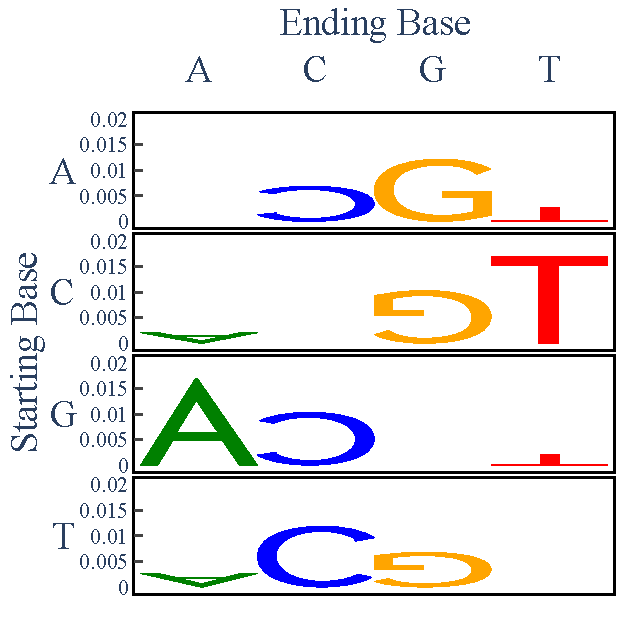
\includegraphics[scale=0.5]{graphics/spectra_Prost-AdenoCA.pdf}
    \caption{Prost-AdenoCA}
    \end{subfigure} \\

    \caption{\textbf{Base substitutions are a rich source of information, manifested by $RE$}}
    \label{fig:apdx_spectra}
\end{figure}
